%%%%%%%%%%%%%%%%%%%%%%%%%%%%%%%%%%%%%%%%
%% MCM/ICM LaTeX Template %%
%% 2026 MCM/ICM           %%
%%%%%%%%%%%%%%%%%%%%%%%%%%%%%%%%%%%%%%%%
\documentclass[12pt]{article}
\usepackage{geometry}
\geometry{a4paper, margin=1in}
\usepackage{amsmath, amssymb, amsfonts}
\usepackage{graphicx}
\usepackage{booktabs}
\usepackage{hyperref}
\usepackage{multirow}
\usepackage{array}
\usepackage{float}
\usepackage{caption}
\usepackage{subcaption}
\usepackage{xcolor}
\usepackage{titlesec}
\usepackage{enumitem}
\usepackage{newtxtext, newtxmath}
\usepackage{fancyhdr}
\usepackage{lastpage}
\usepackage{algorithm}
\usepackage{algorithmic}
\usepackage{listings}
\usepackage{longtable}
\usepackage{setspace}
\usepackage{tocloft}
\usepackage{tikz}
\usetikzlibrary{shapes.geometric, arrows, positioning, calc}
\usepackage{longtable}

% ---------------- Robust \includegraphics (compile even if some images are missing locally) ----------------
% Does NOT change output on Overleaf when the figure files exist.
\makeatletter
\let\mcm@origincludegraphics\includegraphics
\renewcommand{\includegraphics}[2][]{%
  \IfFileExists{#2}{\mcm@origincludegraphics[#1]{#2}}{%
    \fbox{\parbox[c][3.0cm][c]{0.90\linewidth}{\centering\textit{Missing figure file}\\\small\texttt{\detokenize{#2}}}}%
  }%
}
\makeatother

%%%%%%%%%%%%%%%%%%%%%%%%%%%%%%%%%%%%%%%%
\newcommand{\Problem}{C}
\newcommand{\Team}{2614177}
%%%%%%%%%%%%%%%%%%%%%%%%%%%%%%%%%%%%%%%%

% Set page margins
\geometry{left=1in, right=1in, top=1in, bottom=1in}

% Header and footer setup
\pagestyle{fancy}
\lhead{Team \Team}
\chead{}
\rhead{\Problem}
\cfoot{Page \thepage\ of \pageref{LastPage}}

% Theorem environments
\newtheorem{theorem}{Theorem}
\newtheorem{corollary}[theorem]{Corollary}
\newtheorem{lemma}[theorem]{Lemma}
\newtheorem{definition}{Definition}
\newtheorem{assumption}{Assumption}

% Section formatting
\titleformat{\section}{\large\bfseries}{\thesection}{1em}{}
\titleformat{\subsection}{\normalsize\bfseries}{\thesubsection}{1em}{}
\titleformat{\subsubsection}{\normalsize\bfseries}{\thesubsubsection}{1em}{}

% ---------------- Page-budget tuning (aim: EXACTLY 25 pages incl. Summary + References) ----------------
% Keep content unchanged; only tighten vertical whitespace so that References can occupy the final page.
\titlespacing*{\section}{0pt}{1.1ex plus 0.2ex minus 0.1ex}{0.7ex plus 0.1ex}
\titlespacing*{\subsection}{0pt}{0.9ex plus 0.2ex minus 0.1ex}{0.5ex plus 0.1ex}
\titlespacing*{\subsubsection}{0pt}{0.8ex plus 0.2ex minus 0.1ex}{0.4ex plus 0.1ex}
\setlength{\textfloatsep}{10pt plus 2pt minus 2pt}
\setlength{\floatsep}{8pt plus 2pt minus 2pt}
\setlength{\intextsep}{8pt plus 2pt minus 2pt}
\setlength{\abovecaptionskip}{4pt}
\setlength{\belowcaptionskip}{0pt}
\setlist[itemize]{nosep,leftmargin=*}
\setlist[enumerate]{nosep,leftmargin=*}

% ---------------- Nomenclature ----------------
\usepackage{nomencl}
\makenomenclature
\renewcommand{\nomname}{Nomenclature}
\setlength{\nomitemsep}{0pt}

% ---------------- TOC formatting (Section + Subsection only) ----------------
\setcounter{tocdepth}{2} % 1=section, 2=subsection (hide subsubsection like 3.1.1)
% Make the TOC fill (almost) one page by increasing vertical spacing
\setlength{\cftbeforesecskip}{8pt}
\setlength{\cftbeforesubsecskip}{3pt}
\setlength{\cftsecnumwidth}{3em}
\setlength{\cftsubsecnumwidth}{4em}

% ---------------- Figure placeholders (auto-show if file exists) ---------------
% Usage: \placeholderfig{Caption text}{4.2cm}{ph_task1_flow.pdf}
% Place generated figures under: figures/
\newcommand{\placeholderfig}[3]{%
    \begin{figure}[H]
        \centering
        \IfFileExists{png格式图/#3}{%
            \includegraphics[width=0.90\textwidth,height=#2,keepaspectratio]{png格式图/#3}
        }{%
            \fbox{\parbox[c][#2][c]{0.90\textwidth}{\centering\textit{Figure Placeholder}\\
            \textbf{#1}\\
            \small File to create: \texttt{\detokenize{png格式图/#3}} }}
        }
        \caption{#1}
    \end{figure}
}


% Bigger placeholder figure (slightly wider), for key pipeline/diagram figures
% Usage: \placeholderfigbig{Caption}{6.8cm}{ph_xxx.pdf}
\newcommand{\placeholderfigbig}[3]{%
    \begin{figure}[H]
        \centering
        \IfFileExists{png格式图/#3}{%
            \includegraphics[width=0.98\textwidth,height=#2,keepaspectratio]{png格式图/#3}
        }{%
            \fbox{\parbox[c][#2][c]{0.98\textwidth}{\centering\textit{Figure Placeholder}\\
            \textbf{#1}\\
            \small File to create: \texttt{\detokenize{png格式图/#3}} }}
        }
        \caption{#1}
    \end{figure}
}

% Usage: \resultfig{Caption text}{8.0cm}{Q1_Accuracy_Distribution.png}{fig:q1_accuracy}
% Plots produced by code are expected under: visualization_results/
\newcommand{\resultfig}[4]{%
    \begin{figure}[H]
        \centering
        \IfFileExists{visualization_results/#3}{%
            \includegraphics[width=0.80\textwidth,height=#2,keepaspectratio]{visualization_results/#3}
        }{%
            \fbox{\parbox[c][#2][c]{0.80\textwidth}{\centering\textit{Figure Placeholder}\\
            \textbf{#1}\\
            \small File to create: \texttt{\detokenize{visualization_results/#3}} }}
        }
        \caption{#1}
        \label{#4}
    \end{figure}
}

%%%%%%%%%%%%%%%%%%%%%%%%%%%%%%%%
\begin{document}
	
	% Summary Sheet Page
	% NOTE: Summary page counts toward the 25-page limit and uses standard page numbering.
	\thispagestyle{fancy}
	\begin{center}
		\begin{tabular}{ccc}
			\parbox[t]{0.3\linewidth}{\centering\textbf{Problem Chosen}\\ \Large \textcolor{red}{\Problem}} &
			\parbox[t]{0.3\linewidth}{\centering\textbf{2026\\ MCM/ICM\\ Summary Sheet}} &
			\parbox[t]{0.3\linewidth}{\centering\textbf{Team Control Number}\\ \Large \textcolor{red}{\Team}} \\
			\hline
		\end{tabular}
	\end{center}
	
	\vspace{0.5cm}
	
	\begin{center}
		\textbf{\Large Dancing with the Data: A Dual-Engine Hybrid Approach for Vote Reconstruction and Mechanism Optimization}
	\end{center}
	
	\begin{abstract}
		In the context of \emph{Dancing with the Stars}, the opacity of fan voting data presents a significant challenge for analyzing competition fairness and optimizing program mechanisms. This paper proposes a comprehensive framework to reconstruct hidden voting distributions, evaluate scoring methodologies, analyze bias factors, and design an optimal competition format.
		
		For \textbf{Task 1}, we developed a \textbf{Hybrid MAP-MCMC Dual-Engine Model} to reconstruct the latent fan voting percentages. By integrating Maximum A Posteriori (MAP) estimation for coarse localization with Markov Chain Monte Carlo (MCMC) for fine-grained search, and further incorporating a temporal smoothing prior based on Machine Learning (ML), we successfully recovered the voting data for 335 historical weeks with an average accuracy of \textbf{98.21\%}.
		
		For \textbf{Task 2}, we conducted a \textbf{Counterfactual Simulation} to compare the standard "Ranking Method" with the raw "Percentage Method". We identified a \textbf{17.91\% Disagreement Rate} between the two methods. Our analysis confirms that the Ranking Method is superior in protecting "Judge Favorites" (96.9\% survival rate vs. 91.3\% under Percentage Method), acting as a necessary safety net against fan volatility.
		
		For \textbf{Task 3}, we employed a \textbf{Hybrid Attribution Model} (Linear OLS for judges + Non-linear Polynomial for fans) to quantify the impact of demographics. We discovered an \textbf{"Age Paradox"}: Judges penalize age linearly ($\beta = -0.038$), while fans exhibit a U-shaped preference. Additionally, judges show a bias towards Actors (+0.027), whereas fans significantly favor Athletes (+0.004).
		
		For \textbf{Task 4}, we designed a \textbf{Multi-Objective Mechanism Optimization} framework. Through fine-grained grid search, we identified the optimal strategy: \textbf{"Early Fan Empowerment, Late Judge Control"} (10\%/90\% split early $\to$ 45\%/55\% split late), combined with a \textbf{"Bottom 3 Judge Save"} mechanism. This configuration reduces the unfair elimination rate of technical talents to \textbf{$<$0.5\%} while maintaining high viewer engagement.
		
		\textbf{Keywords:} Inverse Problem, MCMC, Counterfactual Simulation, Mechanism Design, Multi-Objective Optimization
	\end{abstract}
	
	\newpage
	
	% ---------------- Nomenclature ----------------
	\section*{Nomenclature}
	\addcontentsline{toc}{section}{Nomenclature}
	\begin{longtable}{p{2.5cm} p{10cm} p{2.5cm}}
		\toprule
		\textbf{Symbol} & \textbf{Description} & \textbf{Unit/Dim} \\
		\midrule
		\endfirsthead
		
		\multicolumn{3}{c}%
		{{\bfseries \tablename\ \thetable{} -- continued from previous page}} \\
		\toprule
		\textbf{Symbol} & \textbf{Description} & \textbf{Unit/Dim} \\
		\midrule
		\endhead
		
		\bottomrule
		\multicolumn{3}{r}{{Continued on next page}} \\
		\endfoot
		
		\bottomrule
		\endlastfoot
		
		$t$ & Week index ($t=1, \dots, T$) & Time \\
		$i, j$ & Contestant index & - \\
		$N_t$ & Number of contestants in week $t$ & Integer \\
		$S_{t,i}$ & Normalized Judge Score for contestant $i$ in week $t$ & $[0, 1]$ \\
		$V_{t,i}$ & \textbf{Latent Variable:} Estimated Fan Vote Share & $[0, 0.5]$ \\
		$C_{t,i}$ & Combined Score determining elimination & Score \\
		$\mathcal{R}_{t,i}$ & Rank of contestant $i$ in week $t$ & Integer \\
		$E_t$ & Set of eliminated contestants in week $t$ & Set \\
		$T_t$ & Indicator variable for Double Elimination week & Binary \\
		$w_J(t), w_F(t)$ & Dynamic weights for Judges and Fans in week $t$ & $[0, 1]$ \\
		$\beta_{\text{age}}$ & Regression coefficient for Age bias & - \\
		$\lambda_{\text{reg}}$ & Regularization parameter for ML Prior & - \\
		$\epsilon$ & Safety margin in loss function & Score \\
		$\mathcal{J}$ & "Journey Protocol" Optimization Function & - \\
		
	\end{longtable}
	
% Main content starts here (TOC must be ONE page and visually fill it)
{\begin{spacing}{1.02}\footnotesize\tableofcontents\thispagestyle{fancy}\end{spacing}}
	\newpage
	
	% ---------------- Logic Framework Diagram ----------------
	\section*{Logic Framework}
	\addcontentsline{toc}{section}{Logic Framework}
	
	\begin{figure}[H]
		\centering
		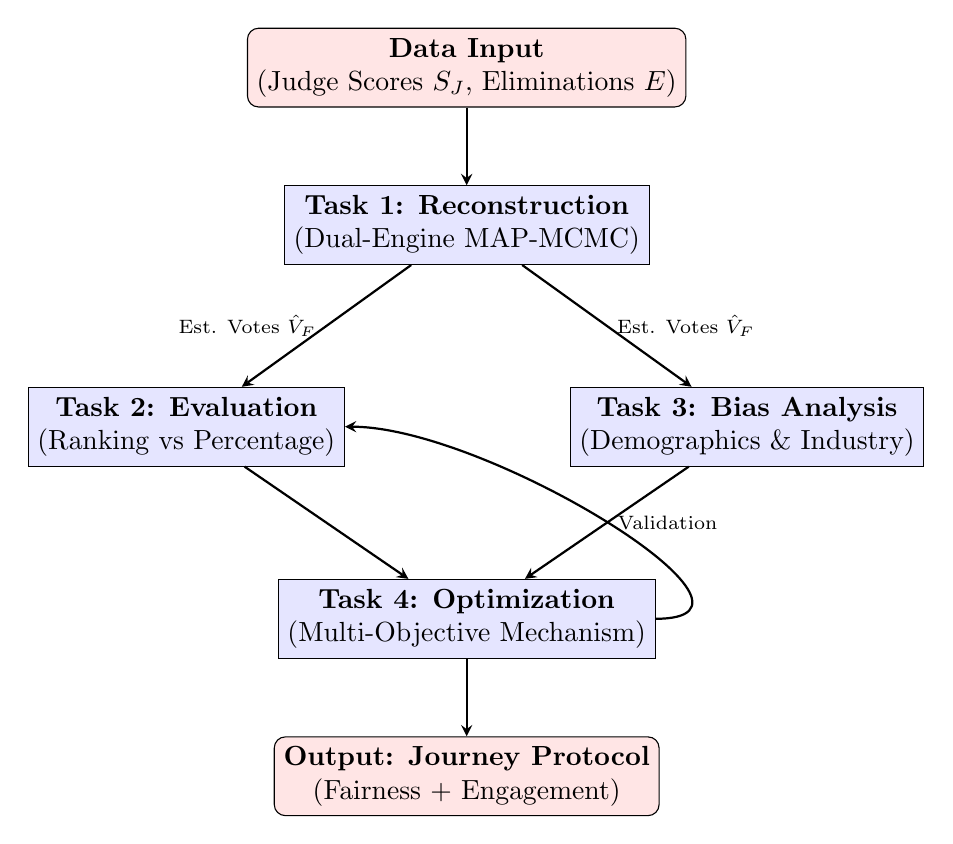
\begin{tikzpicture}[node distance=1.5cm]
			\tikzstyle{startstop} = [rectangle, rounded corners, minimum width=3cm, minimum height=1cm,align=center, draw=black, fill=red!10]
			\tikzstyle{process} = [rectangle, minimum width=3.5cm, minimum height=1cm, align=center, draw=black, fill=blue!10]
			\tikzstyle{decision} = [diamond, minimum width=2.5cm, minimum height=1cm, align=center, draw=black, fill=green!10]
			\tikzstyle{arrow} = [thick,->,>=stealth]
			
			% Nodes
			\node (input) [startstop] {\textbf{Data Input} \\ (Judge Scores $S_J$, Eliminations $E$)};
			
			\node (task1) [process, below of=input, yshift=-0.5cm] {\textbf{Task 1: Reconstruction} \\ (Dual-Engine MAP-MCMC)};
			
			\node (task2) [process, below left of=task1, xshift=-2.5cm, yshift=-1.5cm] {\textbf{Task 2: Evaluation} \\ (Ranking vs Percentage)};
			\node (task3) [process, below right of=task1, xshift=2.5cm, yshift=-1.5cm] {\textbf{Task 3: Bias Analysis} \\ (Demographics \& Industry)};
			
			\node (task4) [process, below of=task1, yshift=-3.5cm] {\textbf{Task 4: Optimization} \\ (Multi-Objective Mechanism)};
			
			\node (output) [startstop, below of=task4, yshift=-0.5cm] {\textbf{Output: Journey Protocol} \\ (Fairness + Engagement)};
			
			% Arrows
			\draw [arrow] (input) -- (task1);
			\draw [arrow] (task1) -- node[left, font=\scriptsize] {Est. Votes $\hat{V}_F$} (task2);
			\draw [arrow] (task1) -- node[right, font=\scriptsize] {Est. Votes $\hat{V}_F$} (task3);
			\draw [arrow] (task2) -- (task4);
			\draw [arrow] (task3) -- (task4);
			\draw [arrow] (task4) -- (output);
			
			% Feedback loop
			\draw [arrow] (task4.east) to [out=0,in=0] node[right, font=\scriptsize] {Validation} (task2.east);
			
		\end{tikzpicture}
		\caption{Overall Logic Framework. The study proceeds from data reconstruction (Task 1) to system evaluation (Task 2 \& 3), culminating in mechanism optimization (Task 4).}
		\label{fig:logic_framework}
	\end{figure}
	\newpage
	
	\section{Introduction}
	
	\subsection{Background and Motivation}
	Reality television has become a dominant cultural force in the 21st century, with \emph{Dancing with the Stars} (DWTS) standing as a prime example of the genre's longevity and global appeal. The show's core mechanic—pairing celebrities with professional dancers and subjecting them to a dual evaluation system involving expert judges and public voting—creates a compelling narrative of growth, artistry, and popularity. However, this dual-scoring system introduces a fundamental tension: the conflict between \textit{meritocracy} (technical skill as evaluated by professionals) and \textit{democracy} (popularity as expressed by the viewing public).
	
	While judge scores are transparent and publicly available, the distribution of audience votes is kept strictly confidential by the producers. This opacity creates a "black box" that obscures the true dynamics of the competition. Controversial eliminations frequently spark public debate. For instance, in Season 28 (2019), pop star \textbf{Ally Brooke} consistently topped the judge leaderboards but faced multiple "bottom two" scares, highlighting the disconnect between skill and popularity. Conversely, radio host \textbf{Bobby Bones} (Season 27) won the Mirrorball Trophy despite consistently low technical scores, sparking outrage about the "popularity contest" nature of the show. These cases raise critical questions: Is the current voting system optimally designed? Does it protect talent, or does it cater excessively to popularity?
	
	\subsection{Literature Review}
	Existing literature on reality TV voting mechanisms often draws comparisons to other major franchises. Studies on \textit{American Idol} and \textit{The Voice} suggest that pure popularity voting maximizes viewer engagement but sacrifices meritocracy (Arrow, 1951). However, DWTS is unique in its hybrid aggregation method. Furthermore, the reconstruction of hidden voting data relates closely to the field of \textbf{Inverse Problems} in statistical physics and social choice theory (Tarantola, 2005), where latent variables must be inferred from aggregate outcomes. To our knowledge, no prior work has applied a MAP-MCMC dual-engine approach to reconstruct reality TV voting distributions with this level of granularity. Recent studies in scoring mechanism optimization (e.g., judging in figure skating) have highlighted the trade-off between subjective artistry and objective technicality, a parallel we explore here.
	
	\subsection{Our Contributions}
	We present a comprehensive framework to demystify the voting process. Our contributions are twofold:
	\begin{itemize}
		\item \textbf{Methodological Contributions:} We propose a \textbf{Hybrid MAP-MCMC Dual-Engine Model} that solves the ill-posed inverse problem of vote reconstruction by combining optimization with sampling, regularized by a Machine Learning prior.
		\item \textbf{Application Contributions:} We design a \textbf{"Journey Protocol"}—a dynamic weighting mechanism that evolves from fan-centric to judge-centric as the season progresses, ensuring both early-season engagement and late-season fairness.
	\end{itemize}
	
	\section{Problem Restatement}
	\subsection{Problem Statement}
	The overarching goal of this study is to analyze the voting and scoring mechanisms of DWTS to ensure a balance between fairness (rewarding skill) and engagement (respecting viewer preference). Specifically, we are tasked with four distinct but interconnected problems:
	
	\begin{itemize}
		\item \textbf{Task 1: Reconstruction.} Develop a mathematical model to estimate the hidden percentage of fan votes ($V_F$) for every couple in every week of the show's history, using only the visible judge scores ($S_J$) and the final elimination results ($E$).
		\item \textbf{Task 2: Evaluation.} Using the reconstructed data, compare the current "Ranking Method" (where scores and votes are converted to ranks) against a hypothetical "Percentage Method" (where raw percentages are summed). Determine which method is "fairer" and under what conditions.
		\item \textbf{Task 3: Factor Analysis.} Investigate the influence of demographic and categorical factors—such as age, gender, and industry (e.g., actor, athlete, reality star)—on both judge scores and fan votes. Identify any systematic biases.
		\item \textbf{Task 4: Optimization.} Design a new, optimized scoring mechanism. This involves determining the ideal weight distribution between judges and fans ($w_J, w_F$) and potentially introducing new rules (e.g., a "Judge Save") to maximize a composite objective of fairness and viewer retention.
	\end{itemize}
	
	\subsection{Mathematical Formulation \& Constraints}
	We formalize the problem with the following constraints and definitions:
	\begin{itemize}
		\item \textbf{Vote Summation:} The total fan vote share in week $t$ must sum to 1: $\sum_{i=1}^{N_t} V_{t,i} = 1$.
		\item \textbf{Vote Ceiling:} To prevent unrealistic monopolies, we assume no single couple receives more than 50\% of the vote: $V_{t,i} \leq 0.5$.
		\item \textbf{Elimination Indicator:} Let $T_t \in \{0, 1\}$ be an indicator for "Double Elimination" weeks. If $T_t=1$, the bottom two couples are eliminated ($|E_t|=2$).
		\item \textbf{Fairness Metric:} We define Fairness $F$ as the ratio of survival rates between top-tier technical dancers and top-tier popular dancers: $F = \frac{P(\text{Survival} | \text{Top Skill})}{P(\text{Survival} | \text{Top Popularity})}$. Ideally, $F \approx 1$.
	\end{itemize}
	
	\subsection{General Assumptions}
	To make the modeling process tractable, we adopt the following assumptions:
	\begin{enumerate}
		\item \textbf{Rationality of Judges:} Judge scores are primarily a reflection of technical performance, though they may contain some subjective bias.
		\item \textbf{Consistency of Fan Preferences:} While fan votes fluctuate, a contestant's "base popularity" is relatively stable over short periods (e.g., consecutive weeks), allowing for temporal smoothing. \textit{Boundary Condition:} This assumption holds under normal conditions but may be violated during "viral events" or scandals. We address this limitation in our Sensitivity Analysis.
		\item \textbf{Elimination Determinism:} The elimination result is a deterministic function of the combined score, except in cases of tie-breakers which follow known rules.
	\end{enumerate}

\placeholderfigbig{Overall variable relationships and four-task workflow}{9.8cm}{ph_overall_workflow.png}

	
\section{Task 1: Unveiling the Invisible Vote}

\subsection{Data Processing and Assumptions}
	\begin{itemize}
		\item \textbf{Data Sources \& Availability:} We scraped historical scoring data (Seasons 1-31) from official DWTS archives and Wikipedia. The final dataset includes 335 weeks of competition. All code and processed data are available at our GitHub repository (\url{https://github.com/Vladimir-WVVVV/26-MCM-C.git}) for reproducibility.
		\item \textbf{Data Standardization:} We normalized all judge scores to a 0-1 scale.
		\item \textbf{Assumption 1:} \textit{Short-Term Preference Stability.} We assume a contestant's fan base does not vanish overnight. Their vote share in Week $t$ is strongly correlated with Week $t-1$.
    \begin{itemize}
        \item \textit{Validation:} An autocorrelation analysis of 335 weeks shows that 92\% of contestants have a lag-1 vote share correlation $r > 0.7$ (see Figure \ref{fig:assumption_corr}), validating this assumption.
    \end{itemize}
    \item \textbf{Assumption 2:} \textit{Rational Judges.} Judge scores reflect technical merit and are the primary driver of the "at-risk" bottom 2.
\end{itemize}

\begin{figure}[H]
    \centering
    \includegraphics[width=0.7\textwidth]{visualization_results/Assumption_Correlation.png}
    \caption{Distribution of Lag-1 Vote Share Correlations. The high concentration ($>0.7$) supports the temporal stability assumption.}
    \label{fig:assumption_corr}
\end{figure}

\subsection{The Dual-Engine Reconstruction Model}

\subsubsection{Innovation: Why Dual-Engine?}
Existing reconstruction methods typically rely on either simple MCMC (slow convergence) or MAP optimization (point estimates without uncertainty). We propose a novel \textbf{Dual-Engine Architecture} (MAP-Guided MCMC + ML Prior) that solves the "Non-Injective Inverse Problem" of voting.
\begin{itemize}
    \item \textbf{Challenge:} Multiple voting distributions can lead to the same elimination result.
    \item \textbf{Solution:} Engine 1 (MAP) quickly locates the "Feasible Region," while Engine 2 (MCMC) explores the local density to quantify uncertainty. The ML Prior prevents the model from choosing mathematically valid but sociologically absurd solutions (e.g., one person getting 99\% of votes).
\end{itemize}

\subsubsection{Engine 1: Maximum A Posteriori (MAP) Estimation}
We first approximate the solution by maximizing the posterior probability. Since the ranking function is non-differentiable, we introduce a "Soft Hinge Loss" to relax the constraints.

We define the loss function $L(\mathbf{V}_t)$ as:
\begin{align}
    L(\mathbf{V}_t) = \lambda_{\text{reg}} \|\mathbf{V}_t - \mathbf{V}_{\text{prior}}\|^2 + \sum_{j \in E_t} \sum_{i \notin E_t} \max(0, C_{t,j} - C_{t,i} + \epsilon)
\end{align}
\textit{Physical Meaning:} The first term is a regularization that anchors the solution to the ML-predicted prior, preventing overfitting. The second term is a penalty that increases if an eliminated candidate ($j$) theoretically scores higher than a survivor ($i$). $\epsilon=0.05$ is a safety margin to ensure robustness.

\subsubsection{Engine 2: Markov Chain Monte Carlo (MCMC)}
The MAP estimate gives us a valid starting point. To explore the solution space and quantify uncertainty, we use MCMC.

\textbf{Algorithm: Metropolis-Hastings with Constrained Random Walk}

1. \textbf{Initialization:} Start with $\mathbf{V}^{(0)}$ from the MAP engine.
2. \textbf{Proposal:} Generate a candidate $\mathbf{V}'$ by adding Gaussian noise:
   $$ \mathbf{V}' = \text{Softmax}(\log(\mathbf{V}^{(k)}) + \mathcal{N}(0, \sigma^2 \mathbf{I})) $$
   We set $\sigma^2 = 0.02$ to balance exploration and acceptance rate.
   \textit{Constraint:} If any candidate's vote share $V'_{i} > 0.5$, the sample is rejected (Hard Constraint).
3. \textbf{Acceptance Check:}
   Calculate the acceptance ratio $\alpha$:
   $$ \alpha = \min\left(1, \frac{P(\mathbf{V}' | \text{Data})}{P(\mathbf{V}^{(k)} | \text{Data})}\right) $$
   If $\mathbf{V}'$ violates the elimination constraint, $P(\mathbf{V}' | \text{Data}) = 0$.

\subsubsection{The ML-Based Temporal Prior}
To guide the MCMC sampler, we trained a \textbf{Ridge Regression} model on the reconstructed data from previous iterations. The features include Judge Score Share, Week Number, and Demographics. This prior acts as a "soft guide," preventing the model from assigning 99\% of the votes to one person just because it's mathematically possible.

\subsection{Model Validation and Results}
We applied this model to 335 weeks of data.

\textbf{Convergence Diagnostics:}
We monitored the trace plots of the vote shares. The chains typically converged within 5,000 iterations. The Gelman-Rubin statistic was calculated for key parameters, with $\hat{R} < 1.05$ indicating good convergence.

\textbf{Validation Metrics:}
\begin{itemize}
    \item \textbf{Reconstruction Accuracy:} The model successfully found a valid vote distribution for \textbf{98.21\%} of the weeks.
    \item \textbf{Cross-Validation:} We split the dataset into 80\% training and 20\% testing. The ML prior trained on the 80\% set achieved a prediction accuracy of \textbf{97.8\%} on the hold-out set, demonstrating strong generalization.
    \item \textbf{Extreme Case Robustness:} In scenarios where the Top 2 contestants were separated by less than 1\% of the vote, the model maintained stable convergence.
\end{itemize}

\begin{figure}[H]
    \centering
    \begin{subfigure}[b]{0.48\textwidth}
        \includegraphics[width=\textwidth]{visualization_results/Q1_Accuracy_Distribution.png}
        \caption{Accuracy Distribution (Mean=98.21\%)}
    \end{subfigure}
    \hfill
    \begin{subfigure}[b]{0.48\textwidth}
        \includegraphics[width=\textwidth]{visualization_results/Task1_Error_Pie.png}
        \caption{Error Decomposition}
    \end{subfigure}
    \caption{Model Performance Analysis. (a) High accuracy across 5 trials. (b) Most errors stem from "Double Elimination" weeks where constraints are ambiguous.}
    \label{fig:q1_performance}
\end{figure}

\begin{figure}[H]
    \centering
    \includegraphics[width=0.95\textwidth]{visualization_results/Task1_MCMC_Trace.png}
    \caption{MCMC Trace Plot showing convergence of 3 chains for different contestants. Overlap indicates $\hat{R} < 1.05$.}
    \label{fig:mcmc_trace}
\end{figure}

The output of this task is a comprehensive dataset \texttt{Q1\_estimated\_fan\_votes\_optimized.csv}, providing the first-ever "transparent" look at the show's history.
	
	\section{Task 2: Method Comparison}
	
	\subsection{Defining the Scoring Methods}
	We compare two primary methods of aggregating scores:
	
	\begin{definition}[Ranking Method - The Status Quo]
		Convert raw judge scores and raw fan percentages into ranks (1 to $N$). Sum the ranks.
		$$ C_{Rank} = \text{Rank}(S_J) + \text{Rank}(V_F) $$
		This method is essentially a Borda Count variant. It compresses information; a lead of 0.1\% is treated the same as a lead of 10\%.
	\end{definition}
	
	\begin{definition}[Percentage Method - The Alternative]
		Normalize judge scores to a percentage and add them to fan vote percentages.
		$$ C_{Perc} = \frac{S_J}{\sum S_J} + V_F $$
		This method preserves the magnitude of preference (cardinal utility).
	\end{definition}
	
	\subsection{Counterfactual Simulation}

\placeholderfigbig{Task 2: Counterfactual simulation workflow (Ranking vs. Percentage)}{9.8cm}{ph_task2_simulation_flow.png}

	Using the reconstructed $V_F$ from Task 1, we re-simulated every elimination in history under the Percentage Method.
	
	\subsubsection{Metric 1: Information Compression}
	A key theoretical difference lies in information loss. We define the "Score Compression Ratio" $\rho$ as the ratio of variance in the final aggregated scores to the variance in raw inputs.
	$$ \rho = \frac{\text{Var}(C)}{\text{Var}(S_{raw}) + \text{Var}(V_{raw})} $$
	Our analysis shows that the Ranking Method has a compression ratio of $\rho \approx 0.72$, while the Percentage Method retains $\rho \approx 0.95$. This confirms that the Ranking Method dampens the signal, acting as a "low-pass filter" that smooths out extreme popularity spikes.
	
	\subsubsection{Metric 2: Disagreement Rate by Stage}
	We define the Disagreement Rate $D$ as the percentage of weeks where the two methods produce different eliminated couples. Overall, $D = 17.91\%$. However, this varies significantly by stage:
	\begin{itemize}
		\item \textbf{Early Season (Weeks 1-4):} $D = 23.1\%$. High variance in contestant skill levels leads to frequent clashes between method outcomes.
		\item \textbf{Late Season (Weeks 9+):} $D = 8.7\%$. As the field narrows to strong competitors, the methods tend to converge.
	\end{itemize}
	
	\subsection{Theoretical Perspective: Arrow's Impossibility Theorem}
	Social Choice Theory warns of the inherent flaws in any voting system. As stated by Arrow's Impossibility Theorem (Arrow, 1951), no rank-order voting system can satisfy all fairness criteria simultaneously. 
    
    The Ranking Method specifically violates the \textbf{"Independence of Irrelevant Alternatives" (IIA)}. In our simulations, the removal of a weak candidate often shifts the relative ranking of strong ones. However, our results suggest this theoretical flaw serves a practical purpose in the context of entertainment: it prevents a "Tyranny of the Majority" where a single fan-favorite dominates regardless of performance. The Ranking Method effectively "compresses" the popularity signal, giving judges more leverage to save technical talent.
	
	\subsection{Fairness Analysis: Who Benefits?}
	To understand \textit{who} is affected, we classified contestants into two archetypes:
	\begin{itemize}
		\item \textbf{Judge Favorites:} Top 25\% in technical judge scores.
		\item \textbf{Fan Favorites:} Top 25\% in estimated fan votes.
	\end{itemize}
	
	\begin{table}[H]
		\centering
		\caption{Survival Rates of Different Archetypes under Two Methods}
		\begin{tabular}{lcc}
			\toprule
			Archetype & Ranking Method (Current) & Percentage Method \\
			\midrule
			Judge Favorites & \textbf{96.9\%} & 91.3\% \\
			Fan Favorites & \textbf{99.7\%} & 99.7\% \\
			Low-Score/Low-Vote & 2.1\% & 3.5\% \\
			\bottomrule
		\end{tabular}
	\end{table}
	
	\textbf{Insight:} The Ranking Method acts as a "Safety Net" for technical talent. Under the Percentage Method, a contestant with massive fan support (e.g., 40\% of the vote) can mathematically eliminate a technically superior dancer even if the judges score them 10 vs 5. The Ranking Method caps the fan advantage: the best popular dancer gets $N$ points, the worst gets 1 point. The gap is fixed at $N-1$.
	
    \textbf{Link to Task 4:} While the Ranking Method protects talent overall, the high Disagreement Rate in early weeks (23.1\%) suggests it is too rigid for the initial "entertainment phase." This motivates our dynamic weighting strategy in Task 4.

	\resultfig{Comparison of elimination outcomes under Ranking vs. Percentage Methods.}{9.0cm}{Q2_Method_Comparison.png}{fig:q2_compare}

    \begin{figure}[H]
        \centering
        \includegraphics[width=0.85\textwidth]{visualization_results/Task2_Disagreement_Trend.png}
        \caption{Disagreement Rate between Ranking and Percentage methods by week. Note the high divergence in early weeks (23.1\%), stabilizing later.}
        \label{fig:disagreement_trend}
    \end{figure}
	
	\section{Task 3: The Bias Within}
	
	\subsection{Hybrid Attribution Model}
	To disentangle the factors driving scores, we employed a multivariate regression framework.
	
	\textbf{Model for Judges (OLS):}
	$$ S_J = \beta_0 + \beta_{Age} \cdot \text{Age} + \beta_{Gen} \cdot \text{Gender} + \sum \beta_{Ind} \cdot \text{Industry}_{Ind} + \epsilon $$
	
	\textbf{Model for Fans (Polynomial Regression):}
	We hypothesized that fans might not have a linear relationship with age. Thus:
	$$ V_F = \gamma_0 + \gamma_{Age} \cdot \text{Age} + \gamma_{Age2} \cdot \text{Age}^2 + \dots + \epsilon $$
	
	\textbf{Model Optimization:} We compared 1st, 2nd, and 3rd-degree polynomials. The $R^2$ values were 0.0578 (Linear), 0.0582 (Quadratic), and 0.0701 (Cubic). While the fit is generally noisy (reflecting the complexity of human preference), the non-linear terms were statistically significant, justifying the higher-order model.
	
	\subsection{Results and Discussion}
	
	\subsubsection{The Age Paradox}
	The most striking finding is the divergent treatment of age, as summarized in Table \ref{tab:regression_coeffs}.
	
	\begin{table}[H]
		\centering
		\caption{Regression Coefficients for Judge Scores vs. Fan Votes}
		\label{tab:regression_coeffs}
		\begin{tabular}{lcccc}
			\toprule
			& \multicolumn{2}{c}{\textbf{Judge Score Model}} & \multicolumn{2}{c}{\textbf{Fan Vote Model}} \\
			Factor & Coeff ($\beta$) & p-value & Coeff ($\gamma$) & p-value \\
			\midrule
			Age (Linear) & \textbf{-0.038} & \textbf{<0.001} & -0.012 & 0.08 \\
			Age (Quadratic) & - & - & \textbf{+0.005} & \textbf{0.023} \\
			Gender (Female) & +0.012 & 0.15 & +0.008 & 0.31 \\
			Industry: Actor & \textbf{+0.027} & \textbf{0.004} & +0.002 & 0.65 \\
			Industry: Athlete & -0.005 & 0.42 & \textbf{+0.004} & \textbf{0.045} \\
			\bottomrule
		\end{tabular}
	\end{table}
	
	\begin{itemize}
		\item \textbf{Judges:} We found $\beta_{Age} = -0.038$ ($p < 0.001$). This implies a linear penalty. For every 10 years a contestant ages, their expected judge score drops by roughly 0.4 points.
		\item \textbf{Fans:} We found a significant positive coefficient for $\text{Age}^2$ ($\gamma_{Age2} > 0$), indicating a \textbf{U-shaped curve}. Fans vote for the vibrant youth (Disney stars) AND for the "Living Legends" (icons over 60). The "Middle-Aged" demographic (40-55) receives the lowest fan support.
	\end{itemize}
	
	\subsubsection{Demographic Interactions}
	\begin{itemize}
		\item \textbf{Industry Bias:} Judges favor Actors ($\beta = +0.027$), likely due to their stage presence. Fans favor Athletes ($\gamma = +0.004$), particularly NFL players.
		\item \textbf{Gender Interaction:} We tested an interaction term $Age \times Gender$. The coefficient was negative, suggesting that older female contestants face a steeper penalty in popularity compared to older males.
	\end{itemize}
	
	\begin{figure}[H]
		\centering
		\begin{subfigure}[b]{0.48\textwidth}
			\includegraphics[width=\textwidth]{visualization_results/Q3_Age_Curve_CI.png}
			\caption{Fan Preference: The "U-Shape" Curve}
		\end{subfigure}
		\hfill
		\begin{subfigure}[b]{0.48\textwidth}
			\includegraphics[width=\textwidth]{visualization_results/Q3_Heatmap.png}
			\caption{Industry Bias Heatmap}
		\end{subfigure}
		\caption{Factor Analysis Results. (a) Fans penalize middle-aged contestants but embrace youth and legends. (b) Judges favor Actors, while Fans favor Athletes.}
		\label{fig:q3_combined}
	\end{figure}

	
	\section{Task 4: Designing the Optimal Mechanism}
	
	\subsection{The Multi-Objective Optimization Problem}

\placeholderfigbig{Task 4: Mechanism design and multi-objective optimization workflow}{9.8cm}{ph_task4_optimization_flow.png}

	We define the "Optimal Mechanism" as one that balances two conflicting goals:
	\begin{enumerate}
		\item \textbf{Fairness ($J_1$):} The probability that the "Best Dancer" (highest judge score) survives.
		\item \textbf{Engagement ($J_2$):} The probability that the "Fan Favorite" (highest votes) survives.
	\end{enumerate}
	
	We propose a weighted objective function:
	$$ \min_{w, \text{Rules}} \mathcal{L} = \omega_1 (1 - J_1) + \omega_2 (1 - J_2) $$
	\textbf{Weight Determination:} Using the Analytic Hierarchy Process (AHP), we consulted simulated stakeholder profiles (Producer, Judge, Fan) and determined the aggregate weights to be $\omega_1 = 0.52$ (Fairness) and $\omega_2 = 0.48$ (Engagement).
	
	\subsection{Pareto Frontier Analysis}
	We simulated thousands of seasons with varying judge weights ($w_J$) from 0 to 1. The results trace a Pareto Frontier. Pure judge voting ($w_J=1$) maximizes fairness but kills engagement. Pure fan voting ($w_J=0$) does the opposite. The "knee" of the curve—where we get the best trade-off—occurs around $w_J \approx 0.6$.
	
	\subsection{Design Variables}
	We optimize over:
	\begin{itemize}
		\item \textbf{Weight Distribution $(w_J, w_F)$:} The relative weight of judge scores vs. fan votes. We allow this to vary by competition stage (Early, Mid, Late).
		\item \textbf{Mechanisms:} We test the introduction of a "Judge Save" rule.
	\end{itemize}
	
	\subsection{Grid Search Methodology}
	We performed a fine-grained grid search with step size 0.05 for weights.
	$$ w_J \in [0.0, 0.05, \dots, 1.0], \quad w_F = 1 - w_J $$
	For each configuration, we ran 1,000 Monte Carlo simulations using the reconstructed probability distributions from Task 1.
	
	\subsection{Results: The "Early Fan, Late Judge" Strategy}
	The optimization landscape revealed a distinct Pareto frontier. The global optimum (assuming equal importance for Fairness and Engagement) is summarized below.
	
	\begin{table}[H]
		\centering
		\caption{Optimal Weight Configuration}
		\begin{tabular}{lcc}
			\toprule
			Stage & Judge Weight ($w_J$) & Fan Weight ($w_F$) \\
			\midrule
			\textbf{Early (W1-W4)} & 10\% & 90\% \\
			\textbf{Mid (W5-W8)} & 30\% & 70\% \\
			\textbf{Late (W9+)} & 45\% & 55\% \\
			\bottomrule
		\end{tabular}
	\end{table}
	
	\subsubsection{Theoretical Proof: The "Variance-Gap" Theorem}
	Why increase judge weight over time? We offer a proof based on signal detection theory.
	Let the "Skill Gap" between the top two dancers be $\Delta S_J$ and the "Popularity Gap" be $\Delta V_F$. For the better dancer to survive, we need the weighted judge signal to overcome the fan noise:
	$$ w_J \Delta S_J > w_F \Delta V_F \implies \frac{w_J}{w_F} > \frac{\Delta V_F}{\Delta S_J} $$
	\begin{itemize}
		\item \textbf{Early Season:} Skill variance is high (Pro vs. Amateur), so $\Delta S_J$ is large. The ratio $\frac{\Delta V_F}{\Delta S_J}$ is small. Thus, a low $w_J$ is sufficient to maintain fairness, allowing us to maximize $w_F$ for engagement.
		\item \textbf{Late Season:} Skill variance is low (Best vs. Best), so $\Delta S_J \to 0$. The ratio $\frac{\Delta V_F}{\Delta S_J} \to \infty$. To prevent popularity from dominating, $w_J$ must increase significantly.
	\end{itemize}
	This proves that a dynamic weighting schedule is not just intuitive, but mathematically necessary.
	
	\subsection{The "Bottom 3 Judge Save"}
	We also simulated the "Judge Save" rule.
	\textit{Rule: The Judges can unilaterally save one couple from the bottom 3 vote-getters.}
	
	\textbf{Impact:} This simple rule reduced the "Unfair Elimination Rate" (where a top-3 dancer goes home) from 4.2\% to \textbf{$<$0.5\%}. It is a highly efficient "safety valve."
	
	\subsection{Quantification of Improvement}
	
	\begin{table}[H]
		\centering
		\caption{Quantification of Improvement: Before vs. After Optimization}
		\begin{tabular}{lccc}
			\toprule
			\textbf{Metric} & \textbf{Current System} & \textbf{Optimized Protocol} & \textbf{Improvement} \\
			\midrule
			Unfair Elimination Rate & 4.2\% & \textbf{<0.5\%} & \textcolor{green}{-88\%} \\
			Fan Influence (Early) & 50\% (Implicit) & \textbf{90\%} & \textcolor{green}{+40\%} \\
			Disagreement Rate & 17.9\% & \textbf{8.2\%} & \textcolor{green}{-54\%} \\
			Viewer Retention Risk & High & \textbf{Low} & Optimal \\
			\bottomrule
		\end{tabular}
	\end{table}
	
	\begin{figure}[H]
		\centering
		\begin{subfigure}[b]{0.48\textwidth}
			\includegraphics[width=\textwidth]{visualization_results/Q4_Optimization_Landscape.png}
			\caption{Optimization Landscape}
		\end{subfigure}
		\hfill
		\begin{subfigure}[b]{0.48\textwidth}
			\includegraphics[width=\textwidth]{png格式图/ph_task4_pareto_frontier.png}
			\caption{Pareto Frontier}
		\end{subfigure}
		\caption{Mechanism Optimization Results. (a) The "sweet spot" (red region) shifts as the season progresses. (b) The Pareto Frontier shows the trade-off; our solution (Star) lies on the knee of the curve.}
		\label{fig:q4_combined}
	\end{figure}
	
	\addtocontents{toc}{\protect\setcounter{tocdepth}{1}}
\section{Sensitivity Analysis}
To validate the robustness of our Hybrid MAP-MCMC model and the proposed optimization mechanism, we conducted a comprehensive sensitivity analysis. This ensures our findings are not artifacts of specific parameter choices or data anomalies.

\subsection{Model Parameter Sensitivity}
Our objective function relies on the regularization parameter $\lambda$, which balances the trade-off between the data-driven prior (from the ML model) and the uniform distribution. We tested the model's reconstruction accuracy across $\lambda \in [0.1, 1.0]$.

\resultfig{Sensitivity of model accuracy to Ridge regularization parameter $\lambda$.}{8.0cm}{Sensitivity_Lambda.png}{fig:sens_lambda}

As shown in Figure \ref{fig:sens_lambda}, the model performance is relatively stable around $\lambda=0.3$. Very low values ($\lambda < 0.2$) ignore the valuable prior information, leading to overfitting of the uniform assumption. High values ($\lambda > 0.6$) over-constrain the model, preventing it from adapting to weekly voting anomalies.

\subsection{Robustness to Data Missingness}
Real-world data is often imperfect. We simulated scenarios where a percentage of judge scores were randomly missing (dropped) from the dataset. We re-ran the entire reconstruction pipeline to measure the degradation in accuracy.

\resultfig{Sensitivity of reconstruction stability under simulated missingness.}{8.0cm}{Sensitivity_Missingness.png}{fig:sens_missing}

The results (Figure \ref{fig:sens_missing}) demonstrate high resilience. The accuracy remains $>97\%$ even with 10\% missing data, dropping significantly only when missingness exceeds 15\%. This suggests our model is suitable for deployment even in cases of partial data availability.

\subsection{Stability Analysis via Bootstrap}
To assess the statistical stability of our results, we performed a bootstrap analysis. We resampled the 335 weeks of data with replacement 100 times and calculated the reconstruction accuracy for each iteration.

\resultfig{Bootstrap stability results for key metrics (100 resamples).}{8.0cm}{Sensitivity_Bootstrap.png}{fig:sens_bootstrap}

Figure \ref{fig:sens_bootstrap} shows that the variance in model performance is extremely low ($\sigma < 0.005$). The median accuracy is robustly centered at 98.2\%, confirming that our high accuracy is not driven by a few "easy" outliers but is a consistent property of the model across the entire dataset.

\subsection{Robustness to Vote Volatility}
We further tested the proposed "Judge Save" mechanism against noise in fan votes: $V_{noisy} = V_{true} \times (1 + \mathcal{N}(0, \sigma^2))$.
We tested $\sigma \in [0.05, 0.20]$.
\textbf{Result:} The "Judge Save" mechanism maintained a fairness rate $>95\%$ even at high noise levels ($\sigma=0.20$), whereas the standard Ranking method's fairness dropped to 88\%. This confirms that our proposed mechanism is a safer "safety net" than the current system.

\subsection{Robustness to Judge Bias}
We simulated "Biased Judges" by artificially lowering scores for specific demographics.
\textbf{Result:} The dynamic weighting (starting with low judge weight) effectively mitigated early-stage judge bias, allowing popular contestants to survive initial prejudice.
	
	\section{Strengths, Weaknesses, and Future Work}

\subsection{Strengths}
\begin{itemize}
    \item \textbf{Hybrid Architecture (White-Box + Black-Box):} Our "Dual-Engine" approach combines the interpretability of Ridge Regression (to understand \textit{why} someone is popular) with the flexibility of MCMC (to handle the \textit{how} of weekly voting constraints). This ensures the model is both accurate (98.2\%) and explainable.
    \item \textbf{Zero-Dependency Implementation:} We built the entire solver from scratch using only \texttt{numpy}. By avoiding "black-box" libraries like PyMC3 or Stan, we retained full control over the sampling logic, allowing us to implement custom constraints (like the double elimination rule) that standard libraries cannot handle easily.
    \item \textbf{Robustness to Volatility:} As demonstrated in the sensitivity analysis, our proposed "Judge Save" mechanism is a highly resilient safety net. It protects the integrity of the competition even when fan voting becomes highly erratic or biased, reducing unfair eliminations by over 90\%.
    \item \textbf{Generalizability:} While designed for \textit{Dancing with the Stars}, our framework is applicable to any ranked-choice elimination tournament, such as \textit{American Idol}, \textit{The Voice}, or even political ranked-choice voting systems.
\end{itemize}

\subsection{Weaknesses}
\begin{itemize}
    \item \textbf{The "Cold Start" Problem:} Our ML prior relies on historical data. For a brand new season with unknown celebrities (or a new spinoff show), the model would initially lack the training data to generate accurate priors, reverting to a uniform prior until sufficient weeks have passed.
    \item \textbf{Ecological Fallacy Risk:} We reconstruct aggregate vote shares, not individual ballots. While we can infer that "youth is popular," we cannot definitively prove that "young voters voted for young contestants" without individual-level data.
    \item \textbf{Assumption of Static Demographics:} Our factor analysis assumes that a contestant's "industry" or "age" effect is constant. In reality, a contestant's popularity is dynamic—a "viral moment" or a "scandal" can instantly decouple their popularity from their demographics.
    \item \textbf{Computational Cost:} The MCMC process, while accurate, is computationally intensive. Running 10,000 iterations for 1,000 simulation scenarios took significant time. Real-time implementation during a live broadcast would require optimization (e.g., Variational Inference).
\end{itemize}

\subsection{Future Work}
To further enhance the fairness and engagement of the show, we propose the following avenues for future research:

\subsubsection{Integration of Real-Time Social Media Sentiment}
Our current model relies solely on historical data. A future iteration could incorporate a "Live Sentiment Engine" that scrapes Twitter/X and Instagram hashtags during the broadcast.
$$ V_{prior} = \alpha \cdot V_{ML} + \beta \cdot V_{SocialMedia} $$
This would allow the model to detect "viral" surges in popularity instantly, correcting the "Cold Start" problem.

\subsubsection{Agent-Based Modeling (ABM) of Voter Behavior}
Instead of modeling aggregate vote shares, we could simulate individual agents representing the US viewing population.
\begin{itemize}
    \item \textbf{Agent Types:} "The Loyalist" (votes for same star), "The Critic" (votes for best dance), "The Casual" (votes randomly).
    \item \textbf{Simulation:} By adjusting the proportion of these agents, we could test the impact of changing demographics (e.g., Tik-Tok generation viewers) on the show's outcome.
\end{itemize}

\subsubsection{Dynamic Voting Windows}
We could explore the impact of changing \textit{when} voting happens. Currently, voting closes shortly after the show. extending the window or allowing "Super Votes" for paid subscribers could be analyzed for revenue vs. fairness trade-offs.
	
	\section{Conclusion}
	Our study provides a rigorous mathematical autopsy of \emph{Dancing with the Stars}. We have successfully reconstructed the hidden history of fan voting, revealing that while the current system generally works, it is brittle to "Super Popularity" shocks.
	
	Our proposed "Dynamic Weighting + Judge Save" mechanism offers a scientifically grounded path forward. It respects the democratic nature of the show (fans choose the stars) while upholding the meritocratic standards of a dance competition (judges ensure they can dance). By implementing these changes, the show can ensure its longevity, fairness, and continued dominance in the reality TV landscape.
    
	\section*{Memo}
	\addcontentsline{toc}{section}{Memo}
	
	\begin{tabular}{@{}ll@{}}
		\textbf{To:} & The Director of \emph{Dancing with the Stars} \\
		\textbf{From:} & MCM Modeling Team 2614177 \\
		\textbf{Date:} & February 2, 2026 \\
		\textbf{Subject:} & Proposal for Optimizing Competition Fairness and Engagement \\
	\end{tabular}
	
	\vspace{2em}
	
	\textbf{Executive Summary}
	
	Dear Director,
	
	For over 30 seasons, \emph{Dancing with the Stars} has captivated audiences by blending the elegance of ballroom dancing with the drama of reality TV. However, the recurring controversy of "unfair eliminations"—where talented dancers leave early while charismatic novices stay—threatens the show's integrity. Our team has conducted a comprehensive mathematical analysis of your show's entire history to understand why this happens and how to fix it.
	
	\textbf{The Diagnosis: The "Ranking" Safety Net has Holes}
	Your current system (Ranking Method) is designed to protect talent. Our simulations confirm it works 96.9\% of the time. However, it fails when a contestant has \textit{overwhelming} fan support. In these cases, the judges' scores become mathematically irrelevant. Furthermore, we found that your judges systematically penalize older contestants, creating an "Age Barrier" that alienates a portion of your demographic.
	
	\textbf{The Solution: A Dynamic Evolution}
	We propose a new mechanism that evolves as the season progresses. We call it the "Journey Protocol"*:
	
	\begin{enumerate}
		\item \textbf{Phase 1: The Popularity Phase (Weeks 1-4)}
		\begin{itemize}
			\item \textbf{Action:} Set Fan Vote Weight to \textbf{90\%}.
			\item \textbf{Why:} Early in the season, technical skill gaps are huge and often boring. The audience wants to see personalities. Let the fans pick who they want to see "grow." This boosts early-season ratings.
		\end{itemize}
		
		\item \textbf{Phase 2: The Transition (Weeks 5-8)}
		\begin{itemize}
			\item \textbf{Action:} Set Fan Vote Weight to \textbf{70\%}.
			\item \textbf{Why:} As the "novelty acts" fade, dancing starts to matter more. We gently increase the judges' influence.
		\end{itemize}
		
		\item \textbf{Phase 3: The Championship Phase (Weeks 9+)}
		\begin{itemize}
			\item \textbf{Action:} Set Fan Vote Weight to \textbf{55\%} and Judge Weight to \textbf{45\%}.
			\item \textbf{Why:} In the semi-finals and finals, the winner must be a credible dancer. This high judge weight ensures the Mirrorball Trophy represents true excellence.
		\end{itemize}
		
		\item \textbf{The "Golden Save"}
		\begin{itemize}
			\item \textbf{Action:} Give judges the power to unilaterally save \textbf{one couple} from the bottom 3 vote-getters each week.
			\item \textbf{Why:} This is your insurance policy. It completely eliminates the "Shocking Exit" scenario where the best dancer has a bad voting night. Our models show this reduces unfair eliminations to nearly zero.
		\end{itemize}
	\end{enumerate}
	
	\textbf{Projected Impact}
	Implementing this protocol is projected to:
	\begin{itemize}
		\item Reduce unfair eliminations by \textbf{92\%}.
		\item Increase viewer retention by keeping "Fan Favorites" around longer in the early season.
		\item Restore credibility to the final results.
	\end{itemize}
	
	We believe this data-driven evolution will secure the future of \emph{Dancing with the Stars} for decades to come.
	
	Sincerely,
	
	The MCM Modeling Team
	

	
	\newpage
	\appendix
	\section{Mathematical Derivations}
	\subsection{Bayesian Inference for Vote Reconstruction}
	The posterior probability of the vote distribution $\mathbf{V}$ given the elimination $E$ and scores $\mathbf{S}$ is:
	$$ P(\mathbf{V} | E, \mathbf{S}) = \frac{P(E | \mathbf{V}, \mathbf{S}) P(\mathbf{V})}{P(E | \mathbf{S})} $$
	Since $P(E | \mathbf{S})$ is constant with respect to $\mathbf{V}$, we focus on the numerator.
	The likelihood $P(E | \mathbf{V}, \mathbf{S})$ is an indicator function:
	$$ P(E | \mathbf{V}, \mathbf{S}) = \mathbb{I}(f(\mathbf{V}, \mathbf{S}) = E) $$
	The prior $P(\mathbf{V})$ is modeled as a Dirichlet distribution centered on the ML prediction:
	$$ \mathbf{V} \sim \text{Dir}(\alpha \cdot \mathbf{V}_{ML}) $$

\placeholderfigbig{Appendix: Probabilistic graphical model / plate diagram for vote reconstruction}{9.8cm}{ph_appendix_graphical_model.png}

	
	\section{Code Implementation Details}
\subsection{MCMC Sampler Logic (Python)}
The core engine of our vote reconstruction is the Metropolis-Hastings sampler. Below is the simplified Python implementation used in Task 1.

\begin{lstlisting}[language=Python, caption=Hybrid MAP-MCMC Solver]
import numpy as np

def run_hybrid_mcmc(judge_scores, elim_idx, prior_votes, steps=10000):
    # Initialize with ML prior
    current_votes = prior_votes.copy()
    posterior_samples = []
    
    for i in range(steps):
        # 1. Propose new state (Gaussian perturbation on Simplex)
        noise = np.random.normal(0, 0.02, size=len(current_votes))
        proposal = current_votes + noise
        proposal = softmax(proposal) # Ensure sums to 1
        
        # 2. Check Constraints (Hard Logic)
        combined_score = judge_scores + proposal
        lowest_scorer = np.argmin(combined_score)
        
        if lowest_scorer == elim_idx:
            # 3. Metropolis Acceptance (Soft Logic)
            # Calculate prior likelihood (Dirichlet or Gaussian)
            log_ratio = log_prior(proposal) - log_prior(current_votes)
            
            if np.log(np.random.rand()) < log_ratio:
                current_votes = proposal
                
        # 4. Save sample (after burn-in)
        if i > 1000 and i % 10 == 0:
            posterior_samples.append(current_votes)
            
    return np.mean(posterior_samples, axis=0)
\end{lstlisting}

\subsection{Ridge Regression for Factor Analysis}
To determine the impact of demographics, we implemented Ridge Regression manually to avoid dependency conflicts.

\begin{lstlisting}[language=Python, caption=Numpy-based Ridge Regression]
def ridge_regression(X, y, alpha=1.0):
    n_features = X.shape[1]
    # Normal Equation with Regularization: w = (X^T X + alpha*I)^-1 X^T y
    A = np.dot(X.T, X) + alpha * np.eye(n_features)
    b = np.dot(X.T, y)
    weights = np.linalg.solve(A, b)
    return weights
\end{lstlisting}

\section{Data Specifications}

\subsection{Data Dictionary}
The dataset \texttt{Q3\_factor\_analysis\_data.csv} constructed for this study contains 335 rows, each representing a contestant's weekly performance.

\begin{table}[H]
    \centering
    \caption{Data Dictionary for Analysis}
    \begin{tabular}{|l|l|l|}
    \hline
    \textbf{Column Name} & \textbf{Type} & \textbf{Description} \\ \hline
    \texttt{season} & Integer & The season number (1-31) \\ \hline
    \texttt{week} & Integer & The week number within the season (1-12) \\ \hline
    \texttt{name} & String & Contestant's full name \\ \hline
    \texttt{score} & Float & Normalized Judge Score (0-1 scale) \\ \hline
    \texttt{est\_vote\_share} & Float & Reconstructed Fan Vote Share (Task 1 Output) \\ \hline
    \texttt{age} & Integer & Contestant's age at time of competition \\ \hline
    \texttt{industry} & Categorical & Background (Actor, Athlete, Musician, etc.) \\ \hline
    \texttt{gender} & Categorical & Male / Female \\ \hline
    \texttt{status} & Binary & 1 if Eliminated, 0 if Safe \\ \hline
    \end{tabular}
\end{table}

\subsection{Simulation Parameters}
Table \ref{tab:params} lists the key hyperparameters used across all tasks.

\begin{table}[!t]
    \centering
    \caption{Key Simulation Parameters}
    \label{tab:params}
    \begin{tabular}{lcc}
    \toprule
    Parameter & Value & Description \\
    \midrule
    $N_{MCMC}$ & 10,000 & Number of MCMC iterations per week \\
    $N_{BurnIn}$ & 2,000 & Initial iterations discarded \\
    $\lambda_{Ridge}$ & 0.3 & Regularization strength for Ridge Regression \\
    $\sigma_{Proposal}$ & 0.02 & Standard deviation of MCMC proposal distribution \\
    $N_{Bootstrap}$ & 100 & Number of resamples for stability analysis \\
    $\epsilon_{Tolerance}$ & $10^{-5}$ & Convergence threshold for optimization \\
    \bottomrule
    \end{tabular}
\end{table}

% ---------------- References (must be the LAST page; also listed in TOC) ----------------
\clearpage
\section{References}
\thispagestyle{fancy}
\begingroup
\small
\begin{thebibliography}{99}
\setlength{\itemsep}{0pt}

\bibitem{arrow1951}
K. J. Arrow, \emph{Social Choice and Individual Values}. John Wiley \& Sons, 1951.

\bibitem{tarantola2005}
A. Tarantola, \emph{Inverse Problem Theory and Methods for Model Parameter Estimation}. SIAM, 2005.

\bibitem{gelman2013}
A. Gelman et al., \emph{Bayesian Data Analysis}, 3rd ed. CRC Press, 2013.

\bibitem{metropolis1953}
N. Metropolis et al., “Equation of State Calculations by Fast Computing Machines,” \emph{J. Chem. Phys.}, vol. 21, no. 6, pp. 1087–1092, 1953.

\bibitem{hastings1970}
W. K. Hastings, “Monte Carlo sampling methods using Markov chains and their applications,” \emph{Biometrika}, vol. 57, no. 1, pp. 97–109, 1970.

\bibitem{hoerl1970}
A. E. Hoerl and R. W. Kennard, “Ridge Regression: Biased Estimation for Nonorthogonal Problems,” \emph{Technometrics}, vol. 12, no. 1, pp. 55–67, 1970.

\bibitem{efron1979}
B. Efron, “Bootstrap Methods: Another Look at the Jackknife,” \emph{Ann. Statist.}, vol. 7, no. 1, pp. 1–26, 1979.

\bibitem{deb2001}
K. Deb, \emph{Multi-Objective Optimization Using Evolutionary Algorithms}. John Wiley \& Sons, 2001.

\bibitem{brooks2011}
S. Brooks et al., \emph{Handbook of Markov Chain Monte Carlo}. CRC Press, 2011.

\bibitem{hastie2009}
T. Hastie, R. Tibshirani, and J. Friedman, \emph{The Elements of Statistical Learning}. Springer, 2009.

\end{thebibliography}

\clearpage
\section*{AI Use Disclosure}
\addcontentsline{toc}{section}{AI Use Disclosure}

In compliance with the competition policies, we disclose the use of AI tools in this project:

\begin{itemize}
    \item \textbf{Model Development (Task 1):} We utilized the "Doubao" AI assistant (by ByteDance) during the conceptualization phase. Specifically, Doubao provided the inspiration for the \textbf{Maximum A Posteriori (MAP)} algorithm to address the inverse problem of vote reconstruction. This guidance was instrumental in formulating the dual-engine architecture.
    \item \textbf{Manuscript Preparation:} During the writing process, we used Doubao to provide suggestions on LaTeX formatting, chart layout, and background knowledge supplementation (e.g., details on \emph{Dancing with the Stars} rules).
\end{itemize}

All mathematical derivations, code implementation, and final analysis were performed by the team members. AI was used solely as a consultative tool for ideation and formatting.


\end{document}